\documentclass[12pt]{article}
\usepackage{graphicx}


\begin{document}


\section*{Introduction}

Term “HPC as a Service” refers to an on demand instantiation of HPC Service in a Cloud. This guide presents a simple “HPC cluster” instantiation procedures in an existing OpenStack based System. “HPC as a service” relies on two main principals to instantiate HPC service 1. Providing pre-build OS images for compute nodes with HPC optimized software and 2. Uses of Cloud-Init to configure and tune HCP services. This recipe provides a simple guides to build HPC optimized OS images, prepare cloud-init recipes and finally instantiate fully functional HPC System using HPC optimized image and cloud-init. For HPC System recipe instantiate HPC master node (aka sms node) and HPC compute nodes using pre-configured OS images. The terms master and SMS are used interchangeably in this guide
OS Images are build using components from OpenHPC software stack. OpenHPC represents an aggregation of a number of common ingredients required to deploy and manage an HPC Linux* cluster including resource management, I/O clients, development tools, and a variety of scientific libraries. These packages have been pre-built with HPC integration in mind using a mix of open-source components. The documentation herein is intended to be reasonably generic,
but uses the underlying motivation of a small, 4-node statefull cluster installation to define a step-by-step
process. Several optional customizations are included and the intent is that these collective instructions can
be modified as needed for local site customizations.
Base Linux Edition: this edition of the guide highlights installation without the use of a companion configuration management system and directly uses distro-provided package management tools for component selection. The steps that follow also highlight specific changes to system configuration files that are required as part of the cluster install process.


\subsection*{TargetAudience}
This guide is targeted at experienced Linux system administrators for HPC environments. Knowledge of
software package management, system networking, PXE booting and OpenStack system software is assumed. Command-line input examples are highlighted throughout this guide via the following syntax:
\begin{quote} 
[sms]\# echo "OpenHPC hello world"

\end{quote}
Unless specified otherwise, the examples presented are executed with elevated (root) privileges. The
examples also presume use of the BASH login shell, though the equivalent commands in other shells can
be substituted. In addition to specific command-line instructions called out in this guide, an alternate
convention is used to highlight potentially useful tips or optional configuration options. These tips are
highlighted via the following format:

\begin{quote}	content...
\small Tip: The solution is to increase the size of the manuals. \{Mark V. Shaney\ 
\end{quote}


\subsection*{RequirementAssumption}

This installation recipe assumes the availability of an OpenStack controller (+ network) node four bare metal nodess. The Controller node serve as central controller for OpenStack services and has all the required OpenStack services installed and configured (i.e. keystone, nova, neutron, ironic along with their dependent services) to provision bare metal nodes with CentOS7.2 in a statefull configuration. 
This recipe is tested with OpenStack Mitaka release with CentOS 7.2. This document provides some examples for installing and configuring OpenStack using Mitaka release of packstack from RedHat®. More detail on using packstack can be found https://www.rdoproject.org/install/quickstart/. 
For power management, we assume that the bare metal node baseboard management controllers (BMCs) are available via IPMI from the chosen controller host. For file systems, we assume that the master server (instantiated during provisioning “HPC as a service”) will host an NFS file system that is made available to the HPC compute nodes.

\begin{figure}
	\centering
	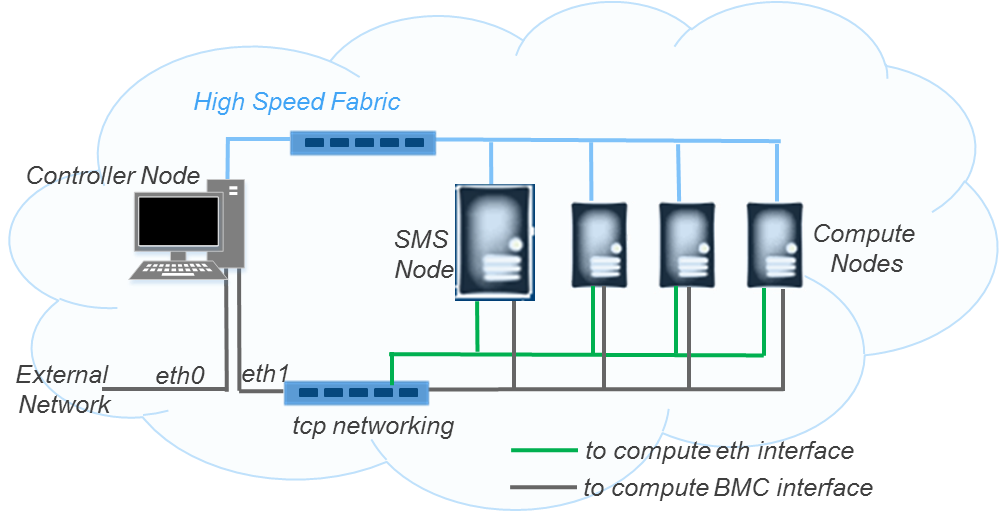
\includegraphics[width=0.7\linewidth]{manifest/figures/HPCaaS-diagram}
	\caption[Openstack node example]{}
	\caption{}
	\label{fig:hpcaas-diagram}
\end{figure}


An outline of the physical architecture discussed is shown in Figure 1 and highlights the high-level
networking configuration. The Controller node requires at least two Ethernet interfaces with eth0 connected to
the external network (public or data center network) and eth1 used to provision and manage the cluster backend (note that these interface names are examples and may be different depending on local settings and OS conventions). Two logical IP interfaces are expected to each compute node: the first is the standard Ethernet interface that
will be used for provisioning and resource management. The second is used to connect to each host’s BMC
and is used for power management and remote console access. Physical connectivity for these two logical
IP networks is often accommodated via separate cabling and switching infrastructure; however, an alternate
configuration can also be accommodated via the use of a shared NIC, which runs a packet filter to divert
management packets between the host and BMC.
In addition to the IP networking, there is a high-speed network (InfiniBand in this recipe) that is also
connected to each of the hosts. This high speed network is used for application message passing and optionally
for Lustre connectivity as well.

\subsection*{Input}
iAs this recipe details installing a cluster starting from bare-metal, there is a requirement to define IP addresses and gather hardware MAC addresses in order to support a controlled provisioning process. These
values are necessarily unique to the hardware being used, and this document uses variable substitution 
(\$fvariableg) in the command-line examples that follow to highlight where local site inputs are required.
A summary of the required and optional variables used throughout this recipe are presented below. Note
that while the example definitions above correspond to a small 4-node compute subsystem, the compute
parameters are defined in array format to accommodate logical extension to larger node counts.
6 Rev: ac5491c
\begin{quote}\small Install Guide (v1.2.1): CentOS7.2/x86 64 + OpenStack + SLURM
\end{quote}

\end{document}
